\documentclass{book}
\usepackage{ctex}
\usepackage{multirow}
\usepackage{graphicx}
\title{标题}
\author{Mary\thanks{E-mail:*****@***.com}\and Ted\thanks{Corresponding author}\and Louis}
% 要生成标题页,title author都不能少
% 在\title、\author 等命令内可以使用\thanks 命令生成标题页的脚注,用\and 隔开多个人名
% 带有目录的tex一般需要编译两次
\begin{document} 
	\maketitle	%生成标题
    \tableofcontents    %生成目录
    \mainmatter		%正文部分,页码为阿拉伯数字格式,从1 开始计数;其后的章节编号正常
    \chapter{一}        % book \chapter \section \subsection三级
        \section{一一}
        gsahd
    \chapter*{二}\addcontentsline{toc}{chapter⟩}{第二章}
    % 加 * 不会在目录中自动生成章节标题,后者\addcontentsline{toc}{<level>}{<title>}手动添加
    % 有区别
        \section{二一}\addcontentsline{toc}{sectio⟩}{第二章第一小节}
        ashjdg
        
        % 在能够被交叉引用的地方,使用\label{⟨label-name⟩} 命令
        % 之后可以在别处使用\ref{⟨label-name⟩} \pageref{⟨label-name⟩} 命令,分别生成交叉引用的编号和页码
        % 在使用不记编号的命令形式(\section*、\caption*、带可选参数的\item 命令等)时不要使用\label 命令,否则生成的引用编号不正确。
        A reference to this subsection\label{sec:this} looks like:‘‘see section~\ref{sec:this} on page~\pageref{sec:this}.’’
        % 使用\footnote 命令可以在页面底部生成一个脚注:
        “天地玄黄,宇宙洪荒。日月盈昃,辰宿列张。”\footnote{出自《千字文》。}
        
        % 有些情况下(比如在表格环境、各种盒子内)使用\footnote 并不能正确生成脚注。我们可以分两步进行,先使用\footnotemark 为脚注计数,再在合适的位置用\footnotetext 生成脚注。
        \begin{tabular}{l}
            \hline
        “天地玄黄,宇宙洪荒。日月盈昃,辰宿列张。”\footnotemark \\
            \hline
        \end{tabular}
        \footnotetext{表格里的名句出自《千字文》。}
        
        
        % 有序和无序列表环境enumerate 和itemize
        % 用\item 标明每个列表项
        % \item 可带一个可选参数,将有序列表的计数或者无序列表的符号替换成自定义的符号。列表可以嵌套使用,最多嵌套四层
        \begin{enumerate}
            \item An item.
            \begin{enumerate}
                \item A nested item.
                \item[*] A starred item.
                \item Another item. \label{itref}
            \end{enumerate}
            \item Go back to upper level.
            \item Reference(\ref{itref}).
        \end{enumerate}
        
        \begin{itemize}
            \item An item.
            \begin{itemize}
                \item A nested item.
                \item[+] A ‘plus’ item.
                \item Another item.
            \end{itemize}
            \item Go back to upper level.
        \end{itemize}
        % 关键字环境description 的用法与以上两者类似,不同的是\item 后的可选参数用来写关键字,以粗体显示,一般是必填的
        \begin{description}
            \item[Enumerate] Numbered list.
            \item[Itemize] Non-numbered list.
        
        \end{description}
        % enumitem 宏包定制各种列表间距。enumitem 宏包还提供了对列表标签、引用等的定制
        
        
        % center、flushleft 和flushright 环境分别用于生成居中、左对齐和右对齐的文本环境。
		\begin{center}
            Centered text using a
            %  \verb 命令(一般用于在正文中插入较短的命令)
            \verb|center| environment.
		\end{center}
		\begin{flushleft}
            Left-aligned text using a
            \verb|flushleft| environment.
		\end{flushleft}
		\begin{flushright}
            Right-aligned text using a
            \verb|flushright| environment.
		\end{flushright}
		% 除此之外,还可以用以下命令直接改变文字的对齐方式:
		% \centering \raggedright \raggedleft
		{\centering Centered text paragraph.
		
		}
		{\raggedright Left-aligned text paragraph.
		
		}
		{\raggedleft Right-aligned text paragraph.
		
		}
		% centering等会影响后面所有的文本(当没有限制作用区域)
		% center 等环境会在上下文产生一个额外间距,而\centering 等命令不产生,只是改变对齐方式。比如在浮动体环境table 或figure 内实现居中对齐,用\centering 命令即可,没必要再用center 环境
		% 上面的centering 如果单纯使用\centering Plain text 之类的来使用,那么三种命令的文本会在同一行显示,且会作用在后面所有的文本(没有限制作用域),可以用上述格式使用,空行必须要有
		
		
		% :quote 用于引用较短的文字,首行不缩进;quotation 用于引用若干段文字,首行缩进。
		% 引用环境较一般文字有额外的左右缩进
		% verse 用于排版诗歌,与quotation 恰好相反,verse 是首行悬挂缩进的
		Francis Bacon says:
		\begin{quote}
            Knowledge is power.
		\end{quote}
            《木兰诗》:
		\begin{quotation}
            万里赴戎机,关山度若飞。
            朔气传金柝,寒光照铁衣。
            将军百战死,壮士十年归。
            
            
            归来见天子,天子坐明堂。
            策勋十二转,赏赐百千强。⋯⋯
		\end{quotation}
        Rabindranath Tagore’s short poem:
		\begin{verse}
            Beauty is truth’s smile
            when she beholds her own face in
            a perfect mirror.
		\end{verse}
		
		% 代码环境verbatim,它以等宽字体排版代码,回车和空格也分别起到换行和空位的作用;带星号的版本更进一步将空格显示成␣
		\begin{verbatim}
		#include <iostream>
		int main()
		{
		std::cout << "Hello, world!"
		<< std::endl;
		return 0;
		}
		\end{verbatim}
		\begin{verbatim*}
		for (int i=0; i<4; ++i)
		printf("Number %d\n",i);
		\end{verbatim*}
		% 要排版简短的代码或关键字,可使用\verb 命令:
		% \verb⟨delim⟩⟨code⟩⟨delim⟩ ⟨delim⟩ 标明代码的分界位置,前后必须一致,除字母、空格或星号外,可任意选择
		\verb|\LaTeX| \\
		\verb+(a || b)+ \verb*+(a || b)+
		% verbatim 宏包优化了verbatim 环境的内部命令,并提供了\verbatiminput 命令用来直接读入文件生成代码环境。fancyvrb 宏包提供了可定制格式的Verbatim 环境;listings 宏包更进一步,可生成关键字高亮的代码环境,支持各种程序设计语言的语法和关键字
		
		
		
		% 表格
		% 直接使用tabular 环境的话,会和周围的文字混排
		\begin{tabular}{|c|}
		center-\\ aligned \\
		\end{tabular},
		\begin{tabular}[t]{|c|}
		top-\\ aligned \\
		\end{tabular},
		\begin{tabular}[b]{|c|}
		bottom-\\ aligned\\
		\end{tabular} tabulars.
		
		\begin{tabular}{lcr|p{6em}}
		% lcr 左对齐 居中 右对齐  都不折行   |表示绘制竖线     p{⟨width⟩} 单元格宽度固定为⟨width⟩,可自动折行
		% 这里参数指:第一列左,第二列中,第三列右,绘制竖线,第四列宽度6em
		% 表格中每行的单元格数目不能多于列格式里l/c/r/p 的总数(可以少于这个总数)
		\hline
		left & center & right
		& par box with fixed width\\
		L & C & R & P \\
		\hline
		\end{tabular}
		% @{}在单元格前后添加任意文本
		\begin{tabular}{@{123} r@{:}lr @{}}
		\hline
		1 & 1 & one \\
		11 & 3 & eleven \\
		\hline
		\end{tabular}
		% \cline{⟨i⟩-⟨j⟩} 用来绘制跨越部分单元格的横线
		\begin{tabular}{|c|c|c|}
		\hline
		4 & &9  \\ \cline{2-2}
		3 & 5 & 7 \\ \cline{1-1}
		8 & 1 & 6 \\ \hline
		\end{tabular}
		% \multicolumn{⟨n⟩}{⟨column-spec⟩}{⟨item⟩}	横向合并单元
		% \multirow{⟨n⟩}{⟨width⟩}{⟨item⟩} 竖向合并单元
		% 纵向合并单元格需要用到multirow 宏包提供的\multirow 命令:
		% ⟨n⟩ 为要合并的列数,⟨column-spec⟩ 为合并单元格后的列格式,只允许出现一个l/c/r 或p 格式
		% ⟨width⟩ 为合并后单元格的宽度,可以填* 以使用自然宽度。
		\begin{tabular}{|c|c|c|}
		\hline
		1 & 2 & Center \\ \hline
		\multicolumn{2}{|c|}{3} &
		\multicolumn{1}{r|}{Right} \\ \hline
		4 & \multicolumn{2}{c|}{C} \\ \hline
		\end{tabular}
		
		\begin{tabular}{ccc}
		\hline
		\multirow{2}{*}{Item} &
		\multicolumn{2}{c}{Value} \\
		\cline{2-3}
		& First & Second \\ \hline
		A & 1 & 2 \\ \hline
		\end{tabular}
		% 嵌套表格
		% 用\multicolumn 命令配合@{} 格式把单元格的额外边距去掉,使得嵌套的表格线能和外层的表格线正确相连
		\begin{tabular}{|c|c|c|}
		\hline
		a & b & c \\ \hline
		a & \multicolumn{1}{@{}c@{}|}
		{\begin{tabular}{c|c}
		e & f \\ \hline
		e & f \\
		\end{tabular}}
		& c \\ \hline
		a & b & c \\ \hline
		\end{tabular}
		
		\newpage
		
\includegraphics[width=12cm]{2}
        \graphicspath{{D:/study/LaTeXandMdandHTML/LaTexWorkspace/short-zn/Image/}}
        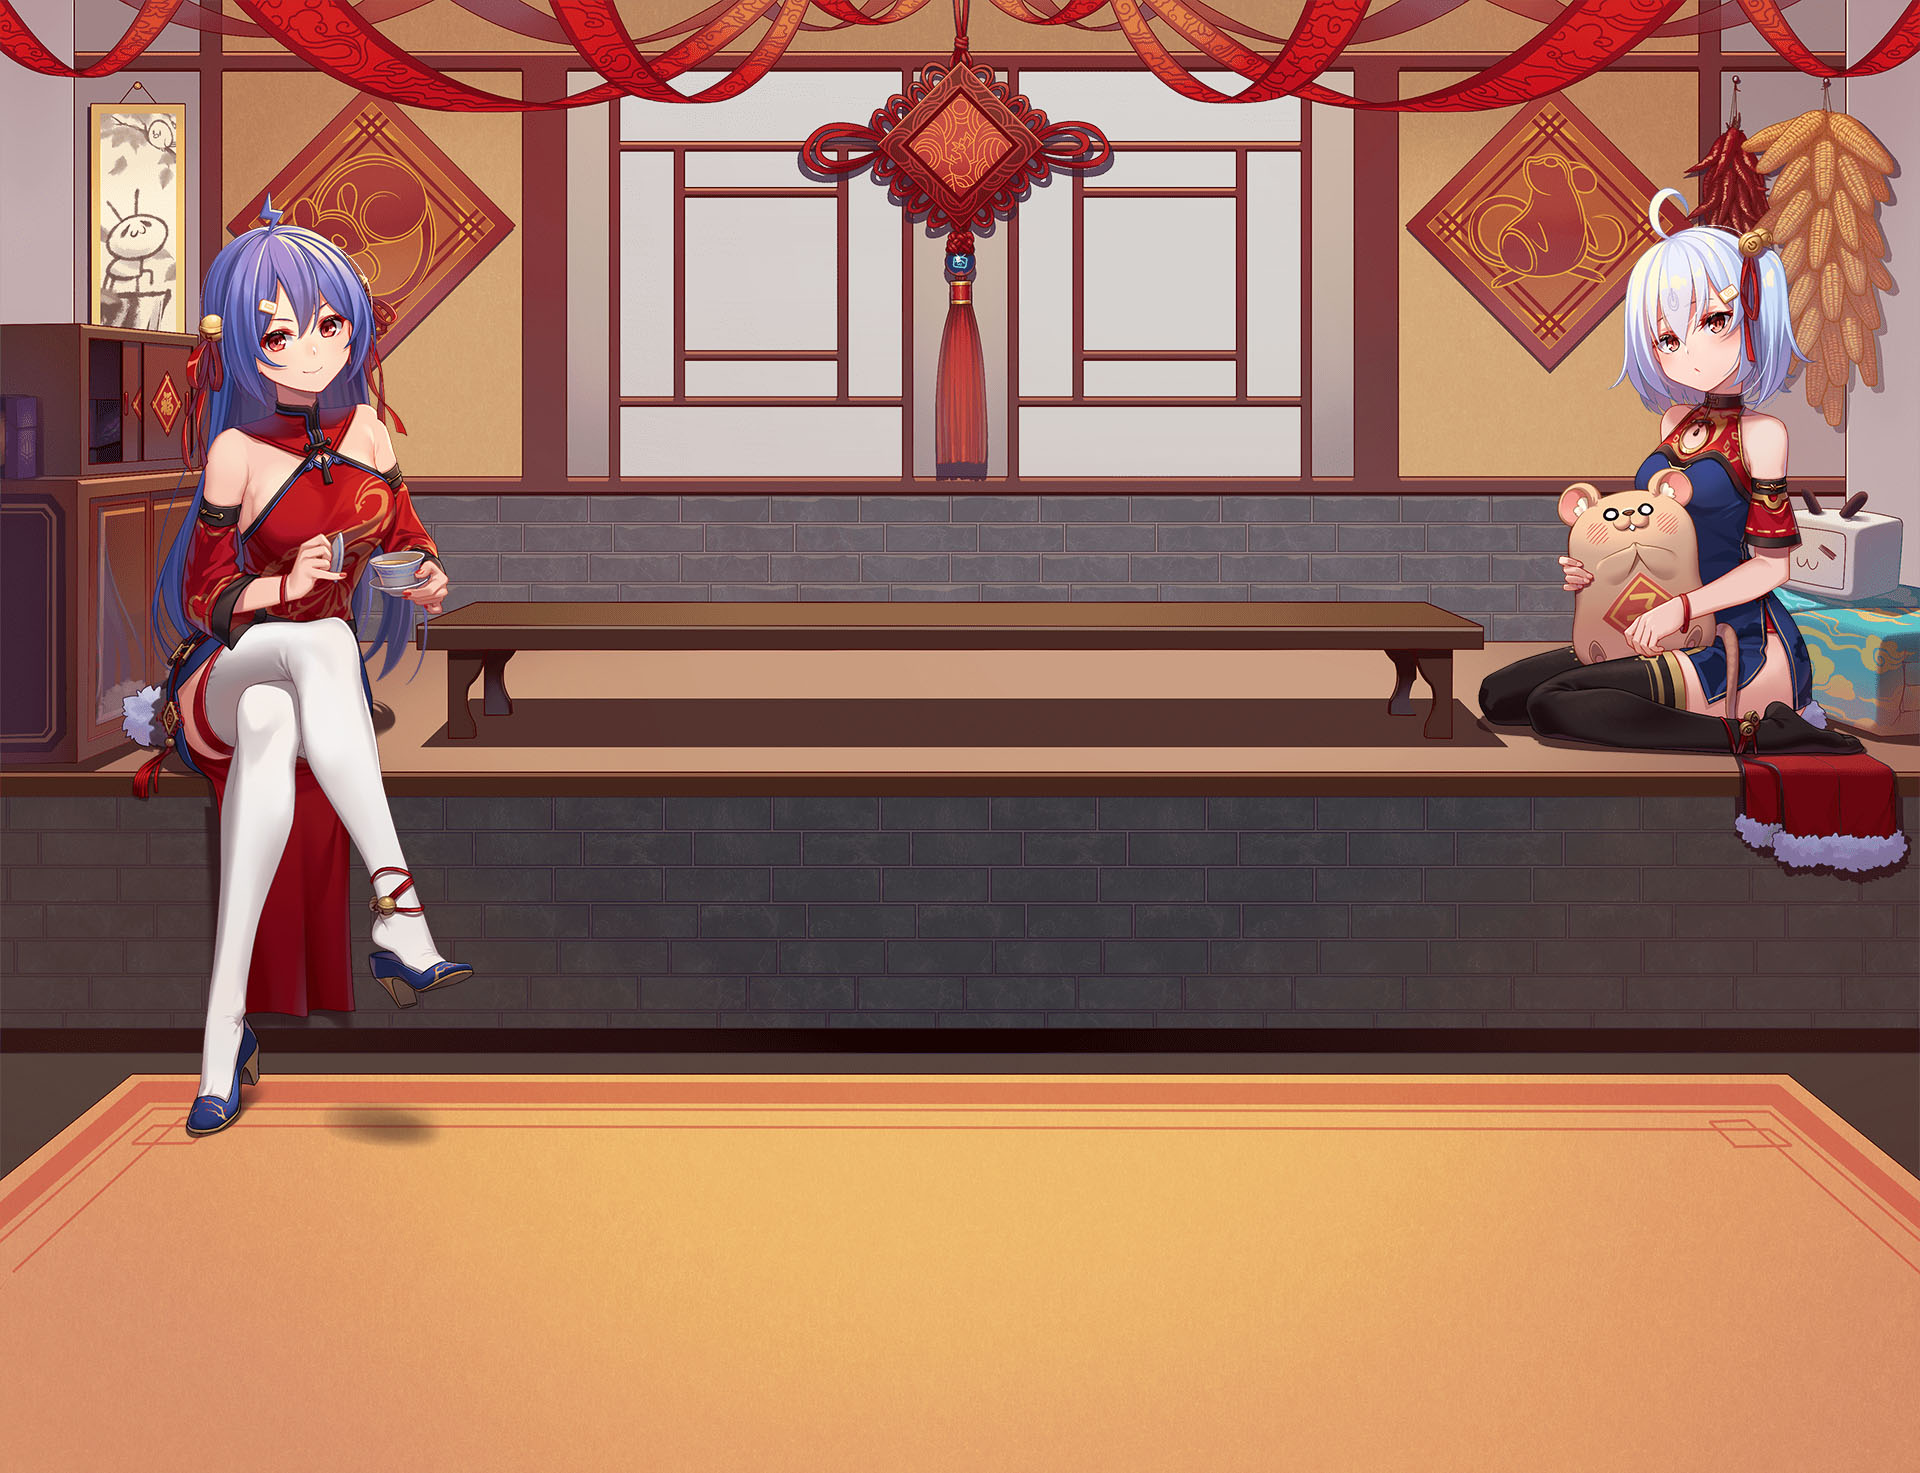
\includegraphics[scale=0.3]{1}
        
\includegraphics[scale=0.1]{3}
        
        
        % 盒子 不允许分段 断行时文字不会从盒子里断开
        |\mbox{Test some words.}|\\
        |\makebox[10em]{Test some words.}|\\
        |\makebox[10em][l]{Test some words.}|\\
        |\makebox[10em][r]{Test some words.}|\\
        |\makebox[10em][s]{Test some words.}|\\
        % 带框的水平盒子
        \fbox{Test some words.}\\
        \framebox[10em]{Text some words .}\\
        \setlength{\fboxrule}{1.6pt}	%边框宽度
        \setlength{\fboxsep}{1em}		% 内边距
        \framebox[10em][r]{Test box}\\
        % 垂直盒子
        三字经:\parbox[t]{3em}%
        {人之初性本善性相近习相远}
        \quad
        千字文:
        \begin{minipage}[b][8ex][t]{4em}
        天地玄黄宇宙洪荒
        \end{minipage}
        % 标尺盒子
        Black \rule{12pt}{4pt} box.
        Upper \rule[4pt]{6pt}{8pt} and
        lower \rule[-4pt]{6pt}{8pt} box.
        A \rule[-.4pt]{3em}{.4pt} line.
        
        
        % 浮动体
        \begin{table}[h]
        	\centering
        	\begin{tabular}{|c|c|c|}
        		\hline
        		直角边a&直角边b&斜边c\\
        		\hline
        		3&4&5\\
        		5&12&13\\
        		\hline
        	\end{tabular}
        	\caption{第一}
        \end{table}
\end{document}
